

\chapter{Microsoft  Kinect Sensor}

\section{Introduction}\label{sec:kinect}

Microsoft released the Kinect device in November 2010 as remote controller for the XBOX gaming console \cite{kinect1}. 
It enables the user to command the XBOX through their voice and body gestures and do not require wearing or using additional accessories to track their movements \cite{kinect1}.
 It features an Red-Green-Blue (RGB) video camera, a depth sensor for 3D representation of environment, multi array microphones for voice recognition and Microsoft software that enables human body recognition \cite{kinect1}. \\
The computer vision society realized that Kinect’s depth sensing capabilities can be used beyond gaming purposes and applications in field of robotics, virtual reality and more started to appear \cite{kinect15}. \\
Kinect drivers that were available for Xbox only, now are available for different platforms such as Linux, Windows and Macintosh. 
On top of them Software Development Kits (SDK) are built, thus enabling development of cross-platform applications.

\subsection{Working  Environment  Introduction }
The system of the present project  consists of three main components:  Hand Detection, preprocessing ,  Gesture Recognition.  This system is built upon  The \textbf{Kinect SDK}  framework the was  used to extract  depth data  from the Kinect sensor.\textbf{C++} was chosen as the main language for this project for its efficient speed and the least memory usage  there is also \textbf{Python} that was used for  evaluating tasks and measure accuracy.


\subsection{Kinect's Features }

Hardware The Kinect has one RGB camera, one depth sensor that consist of one Infra-Red (IR) projector and one IR camera, an array of four microphones and a motorized tilt for changing the field of view \cite{kinect15}. These components are shown in \ref{fig:cam2}

\begin{figure}[H]
\centering
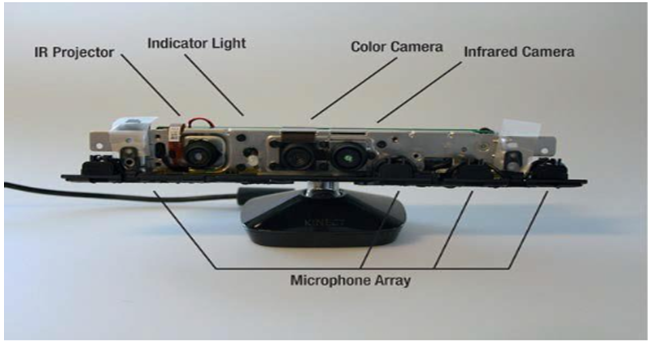
\includegraphics[width=0.53\textwidth]{img/kinectcamera2.png}
\caption{ kinect Hardware }
\label{fig:cam2}
\end{figure}

\textbf{The RGB sensor}  (or video camera) provides 2D view of the scene in three basic colors: Red,Green, and Blue \cite{kinect15} The resolution that can be used is 640x480 pixels or 1280x960 pixels with 32 bits per pixel and the frame rate of 30 frames per second (fps) \cite{kinect15}. \\

\textbf{The depth sensor} \\
– the IR Projector is used to illuminates the scene with structured light while the IR camera observes this illuminated scene and measures the distance of objects from Kinect \cite{kinect15}. As result a depth map is created that gives the distance of objects from the sensor. The depth
map resolution is provided in 320x240 pixels or 640x480 pixels with 16 bits per pixel and an  output frame rate of 30fps \cite{kinect15}. The minimum depth sensor range is from 0.8 meters to a maximum of 4 meters (physical limits). The recommended distance (“Sweet spot” in figure 2.6) is between 1.2m and 3.5m and distances beyond 4m are not recommended since noise get larger \cite{kinect17}. Sun light interferes with infrared light, therefore the depth sensor is not well suited for applications in direct sun light conditions (outdoors)\cite{kinect17} .  

\begin{figure}[H]
\centering
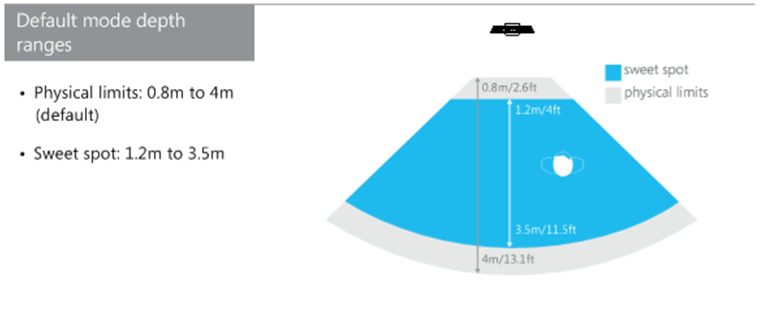
\includegraphics[width=0.8\textwidth]{img/afterworking1.png}
\caption{Kinect depth sensor capabilities}
\label{fig:cam3}
\end{figure}

`\textbf{The motorized tilt}\\
 is used to control the field of view as shown in figure \ref{fig:cam4} and it characteristics are \cite{kinect15} : 
 
\begin{itemize}
\item  Horizontal field of view: 57.5 degree,
\item  Vertical field of view: 43.5 degree,
\item Tilt range: -27 to +27 degree range up and down.

\end{itemize}

\begin{figure}[H]
\centering
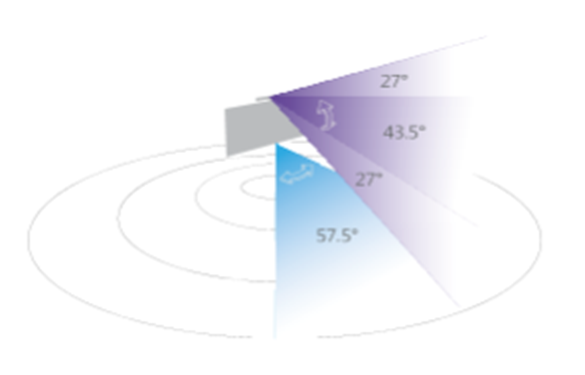
\includegraphics[width=0.6\textwidth]{img/afterworking2.png}
\caption{Kinect depth sensor capabilities}
\label{fig:cam4}
\end{figure}

\textbf{The microphone array} \\
is used for capturing sounds and usually used for speech recognition. It consist of four microphones that enable detection of sound’s source and direction of audio wave \cite{kinect15}. One of them is located at the left of IR projector and the other three microphones are evenly spaced and located at the right of IR camera as shown in \ref{fig:cam5}. The sensor can detect sounds in range of -/+ 50 degree in front of it (\ref{fig:cam5}.a), sound direction in 10 increments  (\ref{fig:cam5}.b) , and offers 20dB (decibel) ambient noise cancellation (\ref{fig:cam5}.c)\cite{kinect17}.

\begin{figure}[H]
\centering
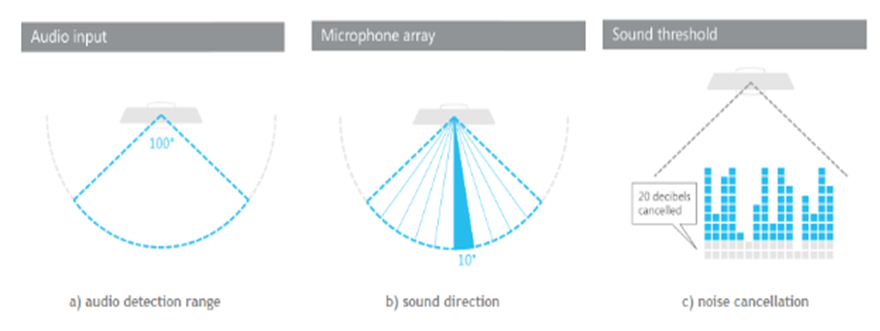
\includegraphics[width=0.8\textwidth]{img/afterworking3.png}
\caption{Kinect sound sensor capabilities a) audio range detection b) sound direction localization c) ambient noise cancellation .
}
\label{fig:cam5}
\end{figure}


\textbf{Skeletal tracking }\\
Skeletal tracking is offered through depth camera. Up to six people can be tracked, while the full skeleton is provided only for two. In full skeleton tracking mode, 20 joints are tracked while in seated mode, half of them (10 joints).The accuracy is larger when the user stands in front of the Kinect, while side standing poses some challenges. Skeletal tracking and two modes are  illustrated in \ref{fig:cam6}.

\begin{figure}[H]
\centering
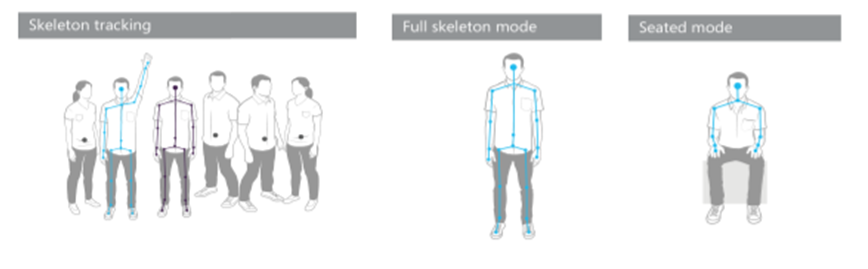
\includegraphics[width=1.0\textwidth]{img/afterworking4.png}
\caption{Skeleton tracking modes through Kinect }
\label{fig:cam6}
\end{figure}

The tracked joint positions are shown in \ref{fig:cam77}
\begin{figure}[H]
\centering
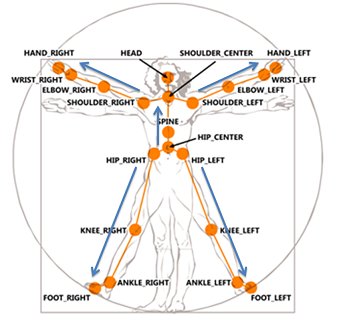
\includegraphics[width=0.4555\textwidth]{img/afterworking5.png}
\caption{Skeleton joint positions offered  through Kinect }
\label{fig:cam77}
\end{figure}

Each skeleton position (body center) and each joint is provided in 3D (x, y, z) coordinates as 
shown in \ref{fig:cam7}. The Kinect is placed at the origin of coordinative system and from Kinect viewpoint: positive Z-axis increases towards the user, positive  Y-axis increases upward and positive  X-axis increases to the left .  

\begin{figure}[H]
\centering
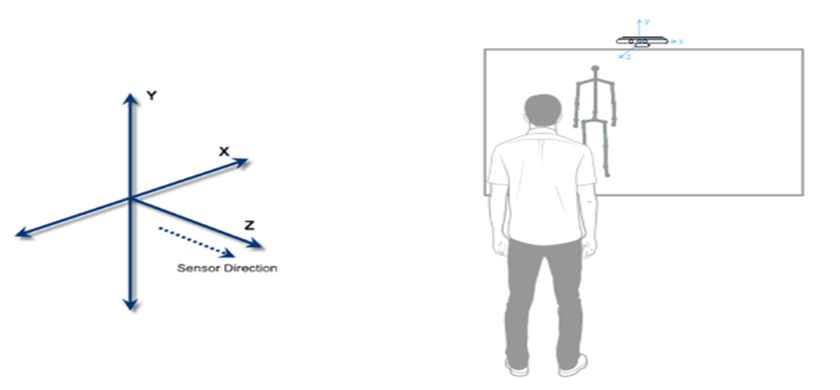
\includegraphics[width=0.7\textwidth]{img/afterworking6.png}
\caption{kinect skeleton coordinate system  }
\label{fig:cam7}
\end{figure}


 
\subsection{linking  kinect SDK with visual studio}

We are using the Kinect SDK version 1.8 and this is how the project is configured. Please note that the developer machine is Windows 7 x86. 
If you are using x64, please change the path accordingly.\\
\textbf{Step 1. } In the Property Manager, right click on the project name and select Add New Project Property\\
Copy C:/Program Files/MicrosoftSDKs/Kinect/v1.0/inc\\
Copy C:/Program Files/MicrosoftSDKs/Kinect/v1.0/lib (you will have both x86 and x64 libraries)\\
\textbf{Step 2}. Configure the project. \\
C/C++ -$>$ General-$>$ add C:/Program Files/Microsoft SDKs/Kinect/v1.8/inc to your Additional Include Directories\\
Linker -$>$ General -$>$ add" C:/Program Files/Microsoft SDKs/Kinect/v1.8/lib/amd64 "  to your Additional Library Directories (if you are configuring for x64, use the amd64 directory)\\
Linker -$>$ Input -$>$ add "Kinect10.lib" to Additional Dependencies\\
\textbf{Step 3}. Compile\\
